\documentclass[a4paper,12pt,twoside]{article}

\usepackage{ucs}
\usepackage[utf8]{inputenc}
\usepackage[T1]{fontenc}
\usepackage[frenchb]{babel}
\usepackage{lmodern}
\usepackage{geometry}
\usepackage{graphicx}
\usepackage{amsmath,amssymb}
\usepackage{float} 
\usepackage{tabularx}
\usepackage{lastpage}           % numérotation
\usepackage{fancyhdr}           % en-têtes
\usepackage{verbatim}
\usepackage{mathpazo}           % police Palatino
\usepackage{xcolor}
\usepackage{listingsutf8}

% En-têtes
\pagestyle{headings}

\title{Systèmes distribués\\
  Make distribué}
\author{Bruno \textsc{Jurkovski}\and Élisabeth \textsc{Rousset}}

% \newenvironment{changemargin}[2]%
% {\begin{list}{}{%
%       \setlength{\listparindent}{\parindent}%
%       \setlength{\itemindent}{\parindent}%
%       \setlength{\leftmargin}{#1}%
%       \setlength{\rightmargin}{#2}%
%     }\item }%
%   {\end{list}}

\begin{document}

\maketitle
\newpage

\tableofcontents

\listoffigures

\newpage

\section*{Introduction}

Ce projet a pour but de programmer une version distribuée de \emph{GNU
  make}. L'exécutable créé sera désigné dans la suite de ce document
par le nom \emph{dmake}. Ce programme possède les fonctionnalités
suivantes :
\begin{itemize}
\item parsing de makefiles simples pouvant contenir des variables
\item distribution des tâches sur un ensemble de noeuds
\item transfert des fichiers nécessaires à l'exécution des tâches sur
  les noeuds concernés
\item exécution des tâches sur les noeuds
\item rapatriement des fichiers créés ou modifiés
\end{itemize}
L'archive fournie contient l'ensemble du code source compilable, les
fichiers tests ainsi que le benchmark utilisé pour l'étude de performances.

\section{Travail réalisé}

Cette section détaille les choix de conception ainsi que
l'installation et le déploiement de \emph{dmake}.

\subsection{Langage}

\emph{Dmake} est programmé en langage C++. Ce langage a été choisi
pour les raisons suivantes :
\begin{itemize}
\item Il s'agit d'un langage objet, ce qui permet d'organiser
  clairement le code et de le rendre lisible.
\item Ce langage possède de nombreuses bibliothèques optimisées qui
  facilitent la tâche du programmeur. En particulier, la gestion
  avancée des \texttt{string} est un atout pour le parsing de
  makefiles. Ce langage paraît donc plus aproprié que le C pour
  programmer \emph{dmake}.
\item Une fois compilé, un exécutable programmé en C++ est nettement
  plus rapide qu'un exécutable équivalent programmé dans un langage
  plus haut niveau comme Java. Ceci est déterminant dans la mesure où
  l'objectif de \emph{dmake} est la performance.
\end{itemize}

\subsection{Bibliothèques}

\emph{Dmake} fait appel aux bibliothèques suivantes pour la gestion
des collections :
\begin{itemize}
\item \texttt{set}
\item \texttt{map}
\item \texttt{vector}
\end{itemize}

Pour la gestion des entrées/sorties, \emph{dmake} utilise :
\begin{itemize}
\item \texttt{cstdio}
\item \texttt{iostream}
\end{itemize}

Les chaînes de caractères sont gérées à l'aide des bibliothèques
suivantes :
\begin{itemize}
\item \texttt{cstring}
\item \texttt{string}
\end{itemize}

Les flux sont gérés à l'aide de :
\begin{itemize}
\item \texttt{sstream}
\item \texttt{streambuf}
\item \texttt{fstream}
\end{itemize}

La vérification de la date de modification/création d'un fichier est
faite grâce à :
\begin{itemize}
\item \texttt{ctime}
\end{itemize}

Le déploiement et l'exécution sur les noeuds utilisent les bibliothèques :
\begin{itemize}
\item \texttt{mpi}
\item \texttt{sys/stat}
\item \texttt{cstdlib}
\item \texttt{unistd}
\item \texttt{algorithm}
\end{itemize}

\paragraph{Remarque}
Le transfert de fichiers et de tâches sur le différents noeuds est
effectué exclusivement avec les primitives de la bibliothèque MPI.

\subsection{Algorithmes}

\paragraph{Graphe de dépendances}

L'exécutable \emph{dmake} crée un graphe de dépendances orienté
acyclique pour représenter les dépendances entre les cibles du
makefile donné en entrée. Nous considérons que le makefile est bien
formée et n'a pas des dépendances cycliques.

\paragraph{Ordonnance des tâches}

Aprés l'obtention du graphe, il faut découvrir l'ordre dans lequel
les tâches seront exécutés. Pour cela, on fait un tri
topologique en utilisant les informations du graphe. Pour envoyer les tâches, 
puis, nous avons seulement besoin de suivre cet ordre et de vérifier si toutes 
les dépendances de ce règle ont été exécutés.

\paragraph{Équilibrage de charge}

Le processus maître conserve la trace de l'état de chacun des esclaves (il stocke le nom de la règle actuelle sur lesquels ils travaillent ou une valeur vide si ils sont libres). Chaque fois qu'un esclave indique à le maître qu'il a terminé une tâche, le maître vérifie si la cible suivante de la liste peut être expédié. Si toutes ses dépendances ont été achevées, le maître envoie la tâche au processus qui l'a demandé.

\subsection{Optimisations}

L'optimisation principale qui a été apportée  pour améliorer les performances de \emph{dmake}
c'est de forcer le noeud central à exécuter la dernière cible.

Tout d'abord, la quantité de communications a été considérablement
réduite. En effet, il a été constaté que de manière générale, la
dernière cible (au sens du graphe de dépendances) utilise l'ensemble
des fichiers crées par les cibles précédentes.

\subsection{Architecture}

Pour le développement de l'application, nous avons découplé de la solution en
trois classes principales: Makefile, DistributedMake et Rule.

\begin{figure}[H]
  \centering
  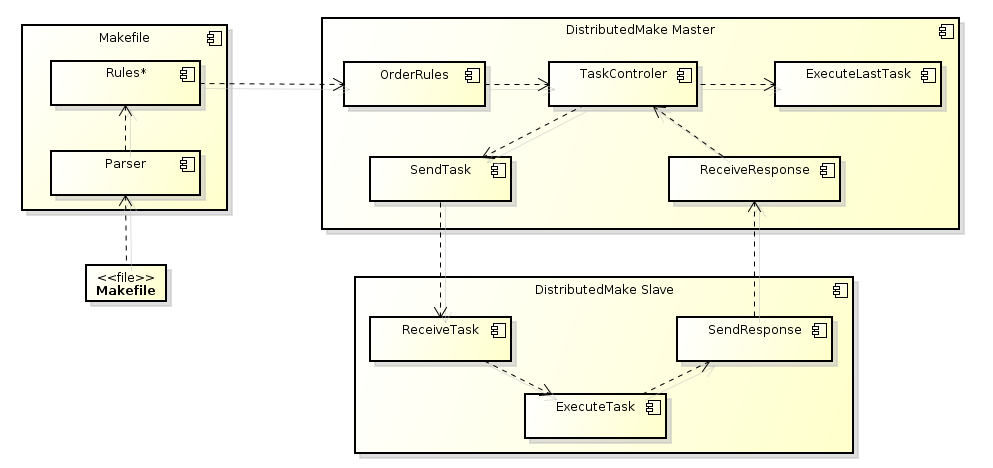
\includegraphics[scale=0.4]{schema.png}
  \caption{Architecture}
  \label{fig:architecture}
\end{figure}

\subsubsection{Rule}

Cette classe contient des informations telles que son nom, une liste des dépendances (de la même classe) et sa liste de commandes à exécuter. Il contient aussi des méthodes pour vérifier si la règle est un fichier (s'il y a un fichier avec le même nom et aucune de ses dépendances du type fichier on été modifiés après lui) et, si elle est, pour vérifier l'heure de sa dernière modification ou s'il a le bit exécutable.

\subsubsection{Makefile}

Cette classe est chargé de la lecture et le parsing d'un fichier Makefile et de la stockage de ses cibles et de son graphe des dépendances.

\subsubsection{DistributedMake}

C'est la classe principale du programme. Il peut être à la fois un maître ou un esclave, selon la façon dont il est appelé dans le programme. Indépendamment du rôle qu'elle joue, elle doit recevoir un paramètre indiquant l'ID de son processus et le nombre total de processus en cours. Ces informations peuvent être récupérées à partir d'un appel MPI.

\paragraph{Maître}

Lorsque initialisé, il crée un tableau de l'état de tous les processus esclaves et entre dans une boucle. Pour chaque processus inactif, il envoie une règle avec ses commandements et les dépendances et marque le nom de la règle dans son entrée dans le tableau. Quand un processus esclave envoie une réponse, il le marque comme étant capable de recevoir de nouvelles tâches.

\paragraph{Esclaves}

Ces processus sont exécutés dans une boucle en attendant pour des tâches. Quand ils le reçoivent, ils l'exécutent et envoient les résultats (fichiers générés) au maître.

\subsection{Installation}

Pour compiler \emph{dmake}, il faut avoir une implémentation de \emph{MPI}.
Dans notres machines, on a utilisé le \emph{OpenMPI}. Pour l'installer, il
suffit d'exécuter la commande suivante :
\begin{verbatim}
> sudo apt-get install openmpi-dev
> sudo apt-get install openmpi-bin
\end{verbatim}

Ensuite, il faut se placer à la racine du
répertoire \texttt{dmake/} puis exécuter la commande :
\begin{verbatim}
> make
\end{verbatim}

\subsection{Déploiement}

Pour déployer \emph{dmake}, il faut d'abord générer la liste des
machines sur lesquelles on souhaite déployer. Pour cela on utilise le
script python \texttt{createMachines.py} en ayant préalablement indiqué
les valeurs souhaitées pour les variables \texttt{startMachine},
\texttt{NUM\_MACHINES}, et \texttt{LAST\_MACHINE} : 
\begin{verbatim}
> python createMachines.py
\end{verbatim}

Ensuite le déploiement lui-même s'effectue à l'aide de
\texttt{mpirun} (qui doit être préalablement installé sur le système). Par exemple, pour lancer \emph{dmake} sur l'un des
exemples fournis dans l'archive, il faut se placer de le dossier
contenant l'exemple puis lancer la commande :
\begin{verbatim}
> mpirun -np NB_CORES -machinefile machines.txt PATH_TO_DMAKE
\end{verbatim}


% Pour déployer \emph{dmake}, il faut tout d'abord regler les paramètre
% de déploiment dans \texttt{dmake.cfg} en indiquant le nombre de
% machines sur lesquelles on souhaite déployer \emph{dmake}, ainsi que 

\section{Tests de performances}

Les performances de \emph{dmake} ont été évaluées à l'aide d'un
benchmark programmé en C++.

\subsection{Méthodologie}

\paragraph{Configuration}
Le benchmark utilise un fichier de configuration
\texttt{benchmark.cfg} dans lequel on précise : 
\begin{itemize}
\item le nombre de fois
\texttt{NUM\_TIMES} qu'est répétée chaque exécution
\item  le nombre minimum \texttt{MIN\_MACHINES}
et le nombre maximum \texttt{MAXIMUM\_MACHINE} de de machines 
sur lesquel on souhaite exécuter les benchmarks
\item le pas \texttt{STEP} concernant le nombre de machines utilisées
  pour l'exécution
\item le type de test \texttt{MAKE\_TYPE} à exécuter. Peut avoit trois valeurs :
	\begin{itemize}
	\item  0 : On n'exécute que le dmake.
	\item  1 : On n'exécute que le make.
	\item  2 : On exécute make et dmake.
	\end{itemize}
\item la localisation \texttt{PATH\_TO\_DMAKE} de \emph{dmake}
par rapport à des tests qui seront exécutés
\item le répertoire \texttt{BASE\_FOLDER} oú se trouvent les tests
\item le nombre de tests à exécuter \texttt{NUM\_BENCHMARKS}
\item la liste des répertoires des tests \texttt{BENCHMARK1}, \texttt{BENCHMARK2}\dots
\end{itemize}

\begin{verbatim}
numTimes NUM_TIMES
machines MIN_MACHINES MAX_MACHINES
step STEP
make MAKE_TYPE
dmakeFolder PATH_TO_DMAKE
baseFolder BASE_FOLDER
numBenchmarks NUM_BENCHMARKS
BENCHMARK1
BENCHMARK2
...
\end{verbatim}

\paragraph{Fonctionnement}

Le programme \emph{benchmark} fonctionne de la manière suivante : pour
chaque fichier test proposé, il exécute successivement \emph{dmake} sur un nombre de
machines allant de \texttt{MIN\_MACHINES} à \texttt{MAX\_MACHINES}
qui est incrémenté de \texttt{STEP} machines à chaque tour. Pour un
fichier de test et un nombre de machines donnés, l'exécution est
répétée \texttt{NUM\_TIMES} fois afin d'obtenir un temps d'exécution moyen
qui soit représentatif. 
Pour chaque fichier test, le temps d'exécution moyen en fonction du
nombre de machines est écrit dans un fichier. Ce fichier est ensuite
utilisé par gnuplot pour générer la courbe correspondante. À cette
courbe est ajoutée une droite horizontale représentant le temps
d'exécution de \emph{GNU make} pour le fichier test considéré. 

\subsection{Conditions expérimentales}

Les test ont été effectués en salle D200. Les machines de cette ont un
seul cœur chacune. La salle était peu occupée
(environ 6 à 10 personnes). Cependant, les tests n'ayant pas tous été
effectués le même jour, les conditions expérimentales ont pu
varier. La charge du réseau notamment a pu être différente selon les
fichiers tests. Les makefiles utilisés pour les tests sont ceux
fournis par le professeur. Ils ont cependant subi les modifications
suivantes : 
\begin{itemize}
\item l'appel à des exécutables présents dans le répertoire courant est
  précédé d'un "./".
\item les fichiers nécessaires à l'exécution d'une cible ont été
  ajoutés dans les dépendances de celle-ci.
\item une cible "clean" a été ajouté pour faire le nettoyage entre deux exécutions.
\end{itemize}

\subsection{Résultats et analyse}

Dans les graphiques suivants, le nombre de machines sur lesquelles est
lancée l'exécution est indiqué en abscisse, tandis que le temps
d'exécution en secondes ou l'accélération comparativement à une
exécution de \emph{GNU make} est indiqué en ordonnées.

\subsubsection{Blender 2.49}

Le benchmark a été réalisé avec un pas de 5 machines, les exécutions
se faisant successivement sur 5, 10, 15 et 20 machines. Chaque
exécution a été répétée 3 fois pour obtenir une moyenne
représentative.

\begin{figure}[H]
  \centering
  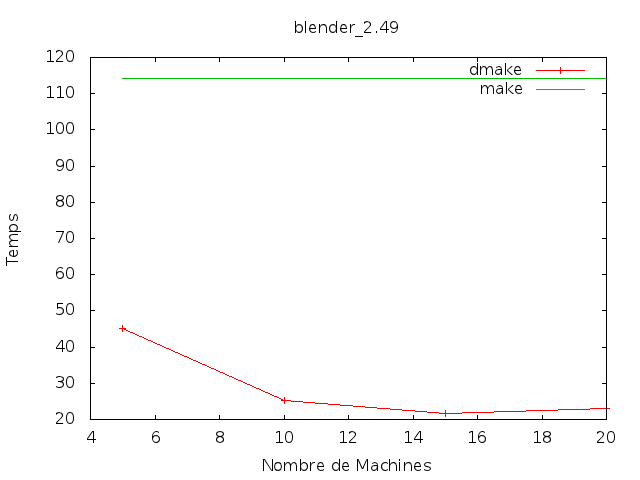
\includegraphics[scale=0.5]{benchmark_blender_2_49_01.png}
  \caption{Blender 2.49}
  \label{fig:blender249}
\end{figure}

On voit ici que l'expérimentation est conforme à nos attentes, car
l'accélération de \emph{dmake} est proche de l'accélération
théorique. Le décalage par rapport à l'accélération théorique peut
être imputée à la partie du code qui est non parallèle. De plus,
l'accélération se stabilise au delà de 20 machine, ce qui s'explique
par le fait que le makefile ne contient que 20 cibles. Les machines
supplémentaires sont donc inutiles. 

\subsubsection{Premier}

Le benchmark a été réalisé avec un pas de 5 machines, les exécutions
se faisant successivement sur 5, 10, 15 et 20 machines. Chaque
exécution a été répétée 3 fois pour obtenir une moyenne
représentative.

\begin{figure}[H]
  \centering
  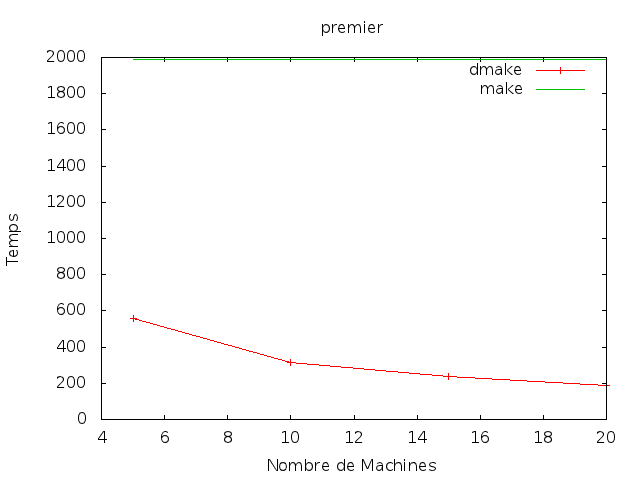
\includegraphics[scale=0.5]{benchmark_premier_01.png}
  \caption{Premier}
  \label{fig:premier}
\end{figure}

De même que précédemment, l'expérimentation est conforme à nos attentes, car
l'accélération de \emph{dmake} est proche de l'accélération
théorique. Ici aussi le décalage par rapport à l'accélération théorique peut
être imputée à la partie du code qui est non parallèle. 

\section*{Conclusion}
On constate que \emph{dmake} est efficace pour des makefiles dont les
tâches sont longues et relativement indépendantes
(cf. \texttt{premier}). En revanche lorsque le temps de communication
n'est plus négligeable devant le temps d'exécution des tâches, les
performances s'effondrent (cf. \texttt{matrix}). On constate le même phénomène lorsque les
tâches sont très dépendantes, car on s'approche alors d'une exécution séquentielle.






\end{document}
